% In this section:
% Someone should be able to build a robot just like ours from the information in this section.
% Include all drawings, specifications, decisions and processes.

\chapter{Design Specification}\label{design specification}\label{section \thechapter}

% Here: Description of what the robot should do/be

\mySection{Robot design and hardware}{writer TBA}
\towrite{hardware}

    \mySubsection{Drawing Mechanism}{\AK}
        The research done into digging mechanisms (Section~\ref{outline:drawing tool}) played a central role during the design phase of the mechanism that would be used on \SandE. A strong material that would have the strength to be dragged through sand was required, with metal being the obvious choice. With regards to the part of the mechanism that was in contact with the sand, this was required to be sharp enough to be able to penetrate the sand to a depth that would leave a sufficient print whilst also not causing too much resistance to be overly restrictive on the motion of the \SandE.\\
        Research into digging mechanisms had shown that multiple teeth dragging through the sand was generally accepted as giving the best results, whether this be through simply using a rake, or having custom built teeth. Consequently three servos would be mounted onto the back of the robot with two teeth on each individual digging component. This meant \SandE would have six points of contact in the sand when trying to leave a print.

        When the building the prototype digging mechanism two pieces of metal wire, both \SI{2.5}{mm} diameter were attached to a \SI{5}{mm} wire using a spot welder. The two pieces of wire that would act as the teeth digging into the sand were then bent using a prong cam so they would be perpendicular to the direction of motion of the robot. During initial testing of this prototype, by mechanically dragging it through sand, it was found that the imprint left was too faint. So it was apparent that a new design would be required with thicker teeth. The prototype however was found to have satisfactory strength so the new version was designed with thicker wire used for the teeth, and the attachment to the robot. would have a smaller diameter. This was in order to make sure the weight of the mechanism doesn't\todo{tense} become excessive as this would jeopardize the ability of the servos to raise and lower the teeth.

        For the updated version, the teeth were created using \SI{5}{mm} metal wire. The wire was bent into shape using a bar bander and then the ends were sharpened using a metal grinder. A thinner piece of \SI{3}{mm} metal wire was used to attach the teeth to the robot. The ground clearance of the robot was measured and a piece of wire was cut using the guillotine that was long enough to reach the  ground. One end of this piece of wire was filed down to fit into the servo using a lathe. A CO_2 welder was then used to attach the two pieces of metal to complete the digging arm. This component performed well in the initial tests so two more versions were         made so the whole digging mechanism was ready to be attached to the robot.


\mySection{Electronics and control systems}{writer TBA}
\towrite{electronics}
    \begin{figure}
        \centering
        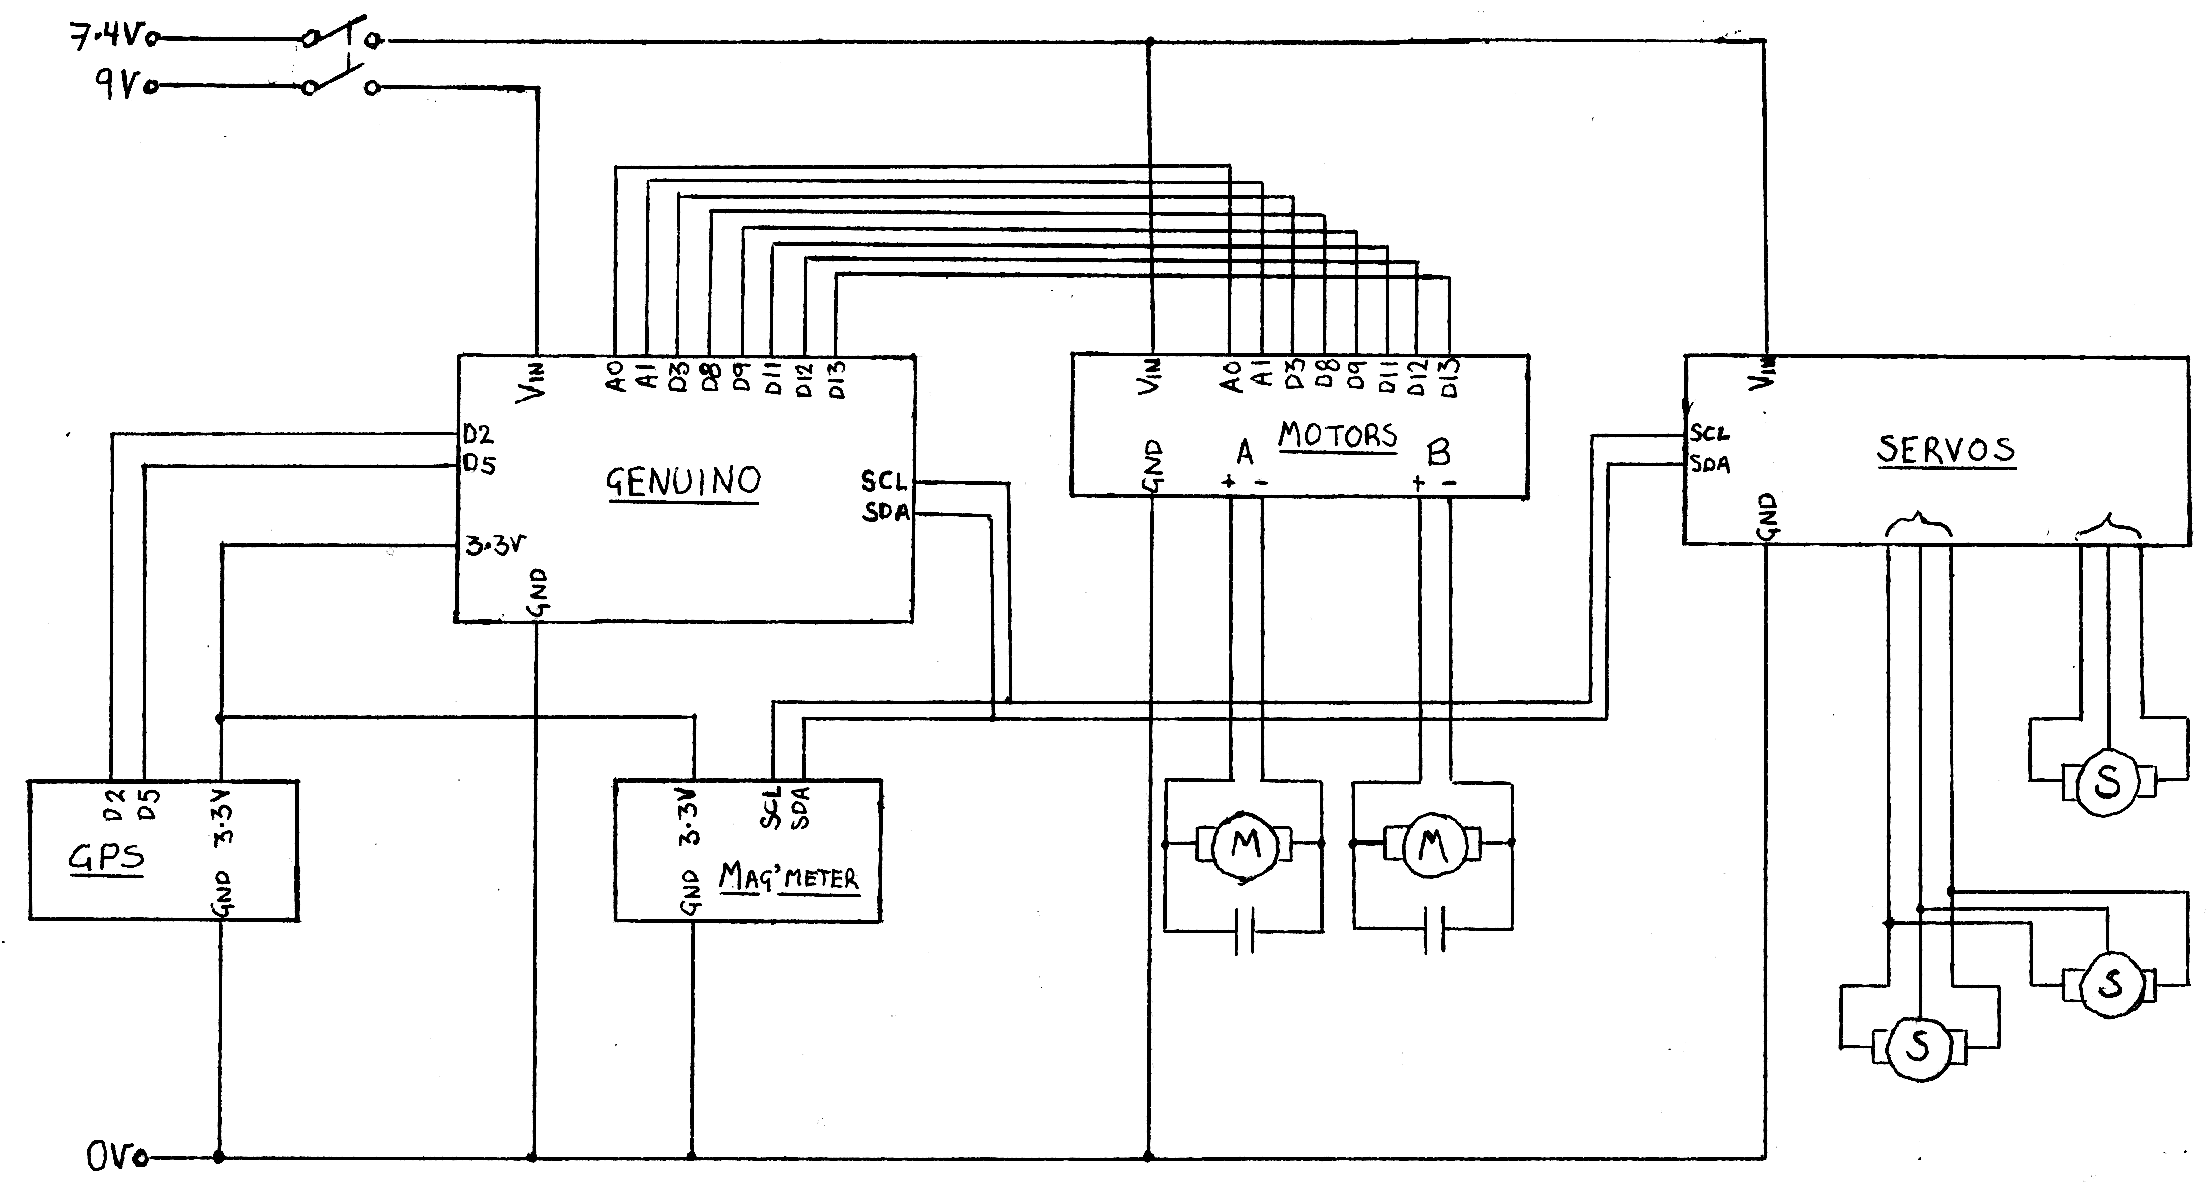
\includegraphics[width=\textwidth]{Files/circuit_diagram}
        \caption{Circuit diagram of the the control system.}
        \label{fig:circuit diagram}
    \end{figure}


\mySection{Software and user interface}{writer TBA}
\towrite{software}


\mySection{Other considerations}{writer TBA}
\towrite{other considerations}
